
\chapter{Introduction}
\label{sec:intro}
We are in the era of autonomous driving: vehicles endowed with a wide variety of sensors, are becoming  capable to navigate in more and more challenging environments.
As humans, the autonomous vehicles exploit vision to perceive and interact with the surrounding environment.
Indeed, many advancements towards the autonomous driving have been achieved thanks to the joint efforts of Computer Vision and Robotics communities.

%Computer Vision aims at extracting meaningful information from images such as the class the subject belongs to, the action happening in the scene or the 3D model of the environment, while Robotics aims at designing robots, or autonomous machines, and at deploying them in the real world.

One of the key aspect in autonomous driving is the awareness of the surrounding provided by the map of the environment. 
To this regard, visual mapping and 3D reconstruction, represent two very active research fields respectively in Robotics and in Computer Vision; both aim at modeling the scene captured through images.
Many works in Robotics focus on the real-time creation of the map while the camera is navigating through an environment, leading to the so called Visual Simultaneous Localization and Mapping (V-SLAM) algorithms. 
On the other hand, Computer Vision researchers tries to recover the  camera poses together with the structure of the map, in a batch fashion, with Structure from Motion (SfM) algorithms.
However, since the proposal of the Parallel Tracking and Mapping (PTAM) algorithm in \cite{klein_murray07} the methods adopted by the two communities became closer and closer, and eventually converged.

SfM and Visual SLAM algorithms build a point-based map of the environment that is often very sparse, except in the case of new semi-dense SLAM, such as LSD-SLAM \cite{engel2014lsd}. 
Only few Dense-SLAM proposals, as DTAM \cite{newcombe2011dtam} or \cite{newcombe2010live}, are able to recover a dense representation of the scene, however they scales badly in large-scale environments, therefor they are not suitable for autonomous driving.

In Computer Vision, the evolution of the Structure from Motion algorithms are the  so called Multi-View Stereo (MVS) algorithms that recover a dense accurate reconstruction of the environment from a set of unordered images. 
MVS algorithms decouple the camera pose estimation and the model computation by delegating the former task to an external algorithm, such as a SfM or a sensor fusion algorithm as \cite{mouragnon_et_al07} or \cite{cucci_matteucci13}, and by focusing on the estimation of an accurate and detailed model of the environment.
As for the early SfM,  Multi-View Stereo has limited its application to off-line, batch processing, indeed no MVS algorithm runs incrementally, since the focus is on accuracy.


In the last decade, many Multi-View Stereo approaches have been proposed; they differ in various aspects, \eg, initialization, optimization procedure, 3D model representation.
Depending on the approach, the scene can be represented by different geometric entities: points, 3D patches, volumes or surfaces.
Points are adopted when the available computational time is limited, \eg, in SLAM, and algorithms relying on 3D patches, which are small 3D portion of surfaces,  show impressive results on highly textured scenes as \cite{furukawa2009reconstructing}. 
These representations cannot be adopted for robot navigation, since they are designed to be sparse, therefore they do not provide a continuous navigable surface.
%All the feature-based and semi-dense SLAM approaches, for computational reasons output such a sparse result, therefor their map are not suitable 

Nowadays, volumetric and mesh-based representations are the most common in the Multi-View Stereo community; they got a boost from the widespread availability of GPU hardware that enables massive parallel processing.
Volumetric algorithms partition the scene into voxels or tetrahedra and estimate which subset represents the free space and which subset represents the matter (Figure \ref{fig:Volumetricc}).
Mesh-based algorithms bootstrap from an initial mesh model of the scene and they evolve its shape in order to minimize the photometric error, \ie, the error between one image and the projection of a second image through the mesh to the first image; we illustrate an example of this projection in (Figure \ref{fig:reproj}.

Volumetric algorithms achieve very accurate results but their application is limited to small scene, since their data structure is not scalable. 
The best trade off between scalability and accuracy is achieved by the mesh-based algorithms which have been proven to score state of the art accuracy \cite{li2015detail} and to reconstruct large-scale scenes \cite{vu_et_al_2012}.

In mesh-based algorithms the initialization represents a crucial aspect.
A widespread initialization is known as visual hull, the reconstruction is the intersection of cones with the vertex in the camera and tangent to the perceived object.
Visual hull needs the knowledge of the silhouette of the objects, which is not a realistic assumption for real world scenarios.
Different approaches have been proposed to initialize a general scene after initialization, by relying on an intermediate volumetric approach, but the process requires human intervention to fix non manifold vertices, because they induce inconsistencies in the mesh refinement.

\begin{figure}
\centering
\begin{minipage}{.5\textwidth}
  \centering
  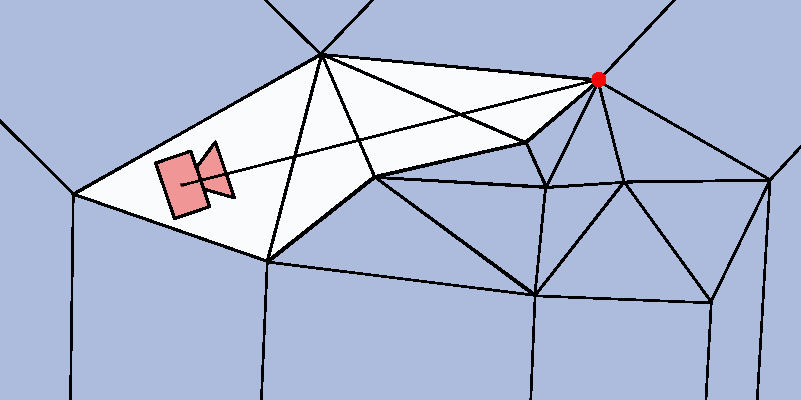
\includegraphics[width=0.5\columnwidth]{./img/spacecarv}
 \caption{Volumetric reconstruction: simple example on 2D case, dark triangles are matter white triangles are free space}
 \label{fig:Volumetricc}
\end{minipage}%
\begin{minipage}{.5\textwidth}
  \centering
  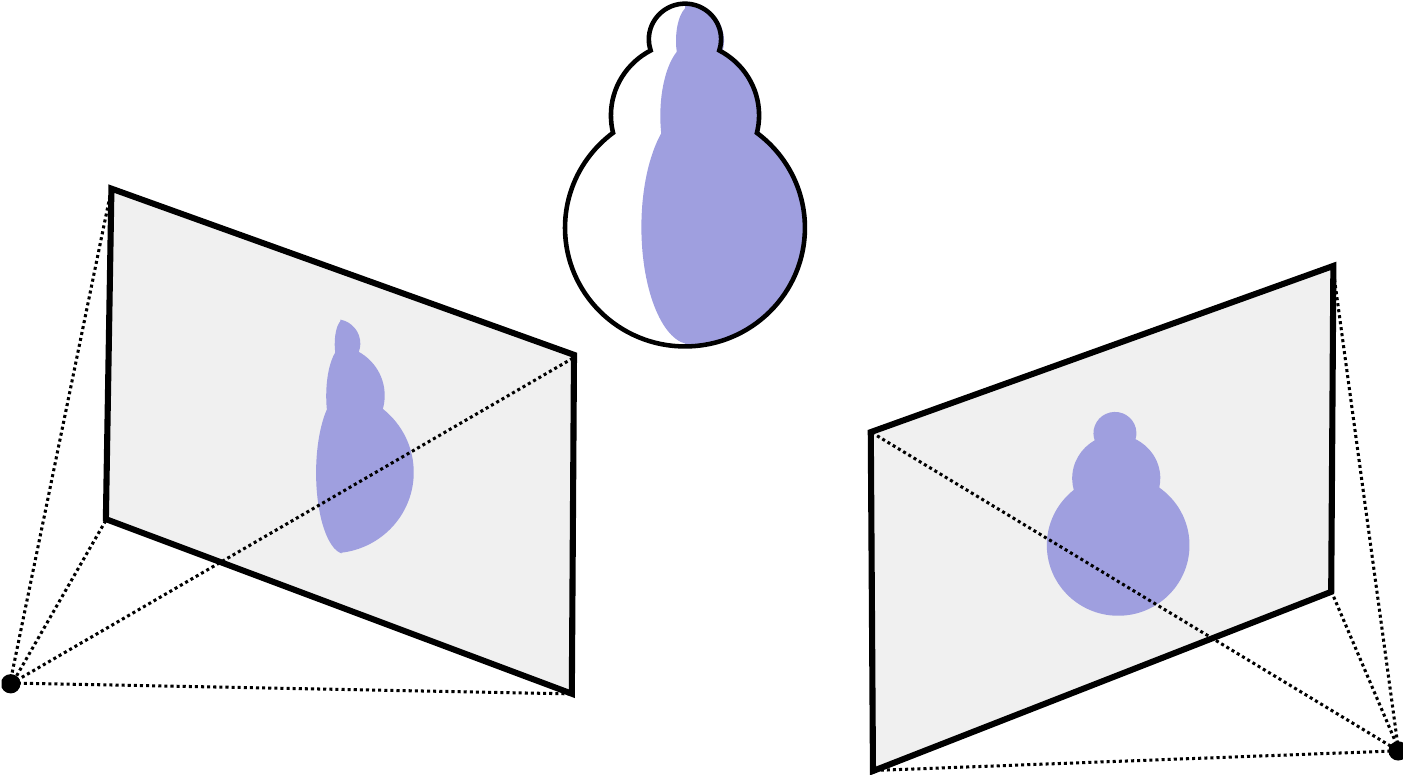
\includegraphics[width=0.5\columnwidth]{./img/reprojOr}
 \caption{Reprojection of image 2 on  image 1 through the model}
 \label{fig:reproj}
\end{minipage}
\end{figure}
%TODO aggiungo immagini e qualche info
\section{Motivations}
To build a bridge between \mvs and dense SLAM we aim at preserving the positive aspects of the two approaches, dropping the drawbacks described thus far. 
On one side the mapping algorithm has to deal with large-scale outdoor environments, as in \mvs or in non-dense SLAM approaches, at the same time it has to estimate an accurate model comparable to the output of \mvs algorithms.
On the other  side, the map has to be estimated incrementally, as in SLAM algorithms.
Indeed, an incremental algorithm is needed whenever an existing map has to be updated with images capturing new regions of the environment, or with new images that add details about an already existing part of the map.
%, as proved by Newcombe \etal \cite{newcombe2011dtam} or by Sch{\"o}ps \etal \cite{schops20153d}. 
For instance incremental processing  is needed during mapping campaigns or drone surveys, where the operators requires to inspect the map while the images are  acquired in order to understand if more data have to be collected, \eg, where details are missing.


The algorithms proposed in the literature are able to cover only part of these requirements.
Many works in \mvs focus on accurate small scale reconstruction; only recently mesh-based approaches have been able to combine scalability and accuracy. They are also able to represent the scene as  a continuous surface, which is very suitable for robotic applications, such as navigation.
However, state-of-the-art \mvs reconstruction pipelines are batch and not fully automatic. 
Classical SLAM provides an incremental estimation of the map, which is however very sparse.
Finally, dense SLAM algorithms are able to estimate incrementally a dense model, but it is limited to small indoor scenes or, in outdoor cases the output accuracy is not comparable to \mvs outputs and the reconstructed surface contains holes where the scene is untextured.

\section{Thesis contributions}
In this thesis we propose the first automatic and incremental pipeline able to build a dense, scalable and manifold mesh, from a set of images.
The mesh representation allows us  to reconstruct  large-scale scenes and continuous meshes.
By keeping the manifold property valid along the whole processing, we are also able to design a completely automatic pipeline, which includes photometric refinement.

The building blocks of our pipeline are essentially two: incremental reconstruction from Sparse Points and incremental mesh refinement.
The former estimates a  manifold mesh from the output of a Structure from Motion algorithm or whatever algorithm which provides camera poses, sparse point clouds and camera-to-point viewing rays.
Incremental reconstruction relies on a volumetric representation obtained through the Delaunay triangulation; each tetrahedron of the triangulation  is voted by the camera-to-point viewing rays and the manifold mesh is extracted as the boundary between those which receive high votes (free space) and those traversed by few or no rays (matter).
We investigated which kind of 3D points are suitable for the Delaunay Triangulation in 3D reconstruction.
We started from two observations: 3D points on real-world edges project mostly on  points belonging to images edges, \ie, the so called 2D edge-points, and edges of the Delaunay triangulation connects near 3D points.
We induced from the two observations that, by estimating the 3D position of 2D edge-points and by building the triangulation upon them, we lead the edges of tetrahedra  to lay on real-world edges.
Therefore, 2D edge-points on the images are the most convenient feature to be reconstructed in 3D.
We also proposed a new voting scheme which improves the accuracy of the reconstruction with respect to the state of the art, and we can now efficiently handle moving point inside the triangulation.

The previous contribution enables incremental refinement. Here, we propose a novel approach to build a dense and detailed map of the environment: as new partial mesh is estimated by the algorithm described thus far, we evolve it photometrically, then we merge it with a mesh representing a new region of the environment trough a novel merging algorithm which is able to keep the manifold property valid.
Our contribution represents a bridge between multi-view stereo and 
dense SLAM: we join the incremental approach of dense SLAM to estimate a  scalable, accurate and continuous model as in state-of-the-art multi-view stereo algorithms. 

Aside from our incremental novel pipeline this thesis presents two other relevant contributions.
We noticed how a manifold mesh estimated from sparse data can sometimes get the refinement process to stuck  in local minima or to converge slowly to the solution. 
We investigated how to overcome this issue by improving the accuracy of  the initialization such that it becomes closer to the real solution.
By adding few accurate 3D points to the sparse point clouds, we significantly speed up the convergence and improve the accuracy of the refinement.
For this purpose, we sweep the initial mesh in the space and we extract a new 3D point where the photometric matching score induced in a pair of camera is very high, which likely means that this point belongs to the real scene.

Moreover, since lidar data are often available together with images in autonomous driving applications, we tested and extended our mapping pipeline to work with hybrid lidar and image data.
We propose a complete mapping framework  that leverages on the high accuracy of the 3D lidar data and on the appearance and density of the images.
By detecting and removing the moving points from lidar point clouds, we reconstruct the map of the scene with our reconstruction algorithm and we are able to refine it by neglecting the moving objects from the photometric optimization. Finally we recover a full textured map where moving points where filtered out.



\section{Thesis outline}

The thesis is organized in three parts. 
In the first part we provide all the background materials needed to understand the contributions of the thesis.
\begin{itemize}
 \item Chapter \ref{ch:computational} gives an overview of the computational geometry tools we use in particular to describe ho we reconstruct a manifold mesh.
 \item Chapter \ref{ch:camera} contains the classic definitions of pin-hole camera and the geometry behind the  multi-view setting, we also present how to formulate the pin-hole model in OpenGL, which adopts different conventions with respect the classical one.
\end{itemize}

The second part of the thesis presents an overview on incremental reconstruction and it presents the main contribution of this thesis.
\begin{itemize}
 \item Chapter \ref{ch:soa} reviews the state of the art in mapping and Multi-View Stereo, focusing on the incremental reconstruction and on dichotomy between the Robotics and  Computer Vision algorithms propose to solve the same mapping problem from two different perspectives
 \item Chapter \ref{ch:incrDenseRef} shows the incremental manifold reconstruction algorithm from a sparse point:  we focus on three contributions: the novel choice of the points adopted to build the volumetric representation of the scene through Delaunay Triangulation; the novel voting heuristic that prevents the creation of most artifacts in the mesh and the novel approach to manage moving points inside the triangulation.
 \item Chapter \ref{ch:incrDenseRef} illustrates the complete novel pipeline we propose to build incrementally a dense mesh on the environment; we focus in particular on the novel merging algorithm and on the refinement process.
\end{itemize}

In the third part of the thesis we illustrate our contribution aside the incremental algorithm, which are closely related to the mesh-based reconstruction.

\begin{itemize}
 \item Chapter \ref{ch:sweeping} shows our novel mesh sweeping algorithm that adds new accurate 3D points to the reconstructed mesh in order to  improve the convergence and the accuracy of the refinement process.
 \item Chapter \ref{ch:laser} presents our approach extended to work with lidar data: we explain how we remove the moving point from the lidar point cloud and how we leverage on this information to estimate a refined and textured mesh.
\end{itemize}

% In Chapter \ref{ch:further} we finally show some further experiments in which our algorithm plays a major role, in particular we show how the dense map can be adopted to localize a camera.














